\section{System Overview}
\label{sec:overview}

\subsection{Requirements}
The proposal set the following requirements for the capstone vessel:
\begin{enumerate}
\item Accept an ordered list of GPS waypoints from an operator and sail
between them without human input, tacking when a leg lies in the no-go zone.
\item Allow manual remote control from the ground station as a fallback.
\item Report position, heading, wind, actuator states, and battery status to
the ground station over a long-range, low-power radio link.
\item Remain stable and watertight in the wind and chop of local reservoirs.
\item Minimize actuator power so that the design scales to long missions.
\end{enumerate}

\subsection{Architecture}
Fig.~\ref{fig:boat} shows the assembled vessel and Fig.~\ref{fig:block} its
electrical and software architecture. All computation runs on one
NUCLEO-H755ZI-Q development board. The STM32H755's Cortex-M7 core (CM7) reads
every sensor and runs planning, control, and mode logic under FreeRTOS, while
its Cortex-M4 core (CM4) runs only the LoRa radio. The two cores exchange
telemetry and commands through shared memory (Section~\ref{sec:sw}). The hull
carries two deck hatches: the forward hatch gives access to the mast step and
sail-angle encoder, and the aft hatch holds the electronics enclosure. The
wind vane and rudder servo are mounted on the aft deck and transom.
Table~\ref{tab:specs} lists the principal dimensions, taken from the computer-aided design (CAD) model unless noted.

\begin{figure*}[!t]
\centering
\subfloat[]{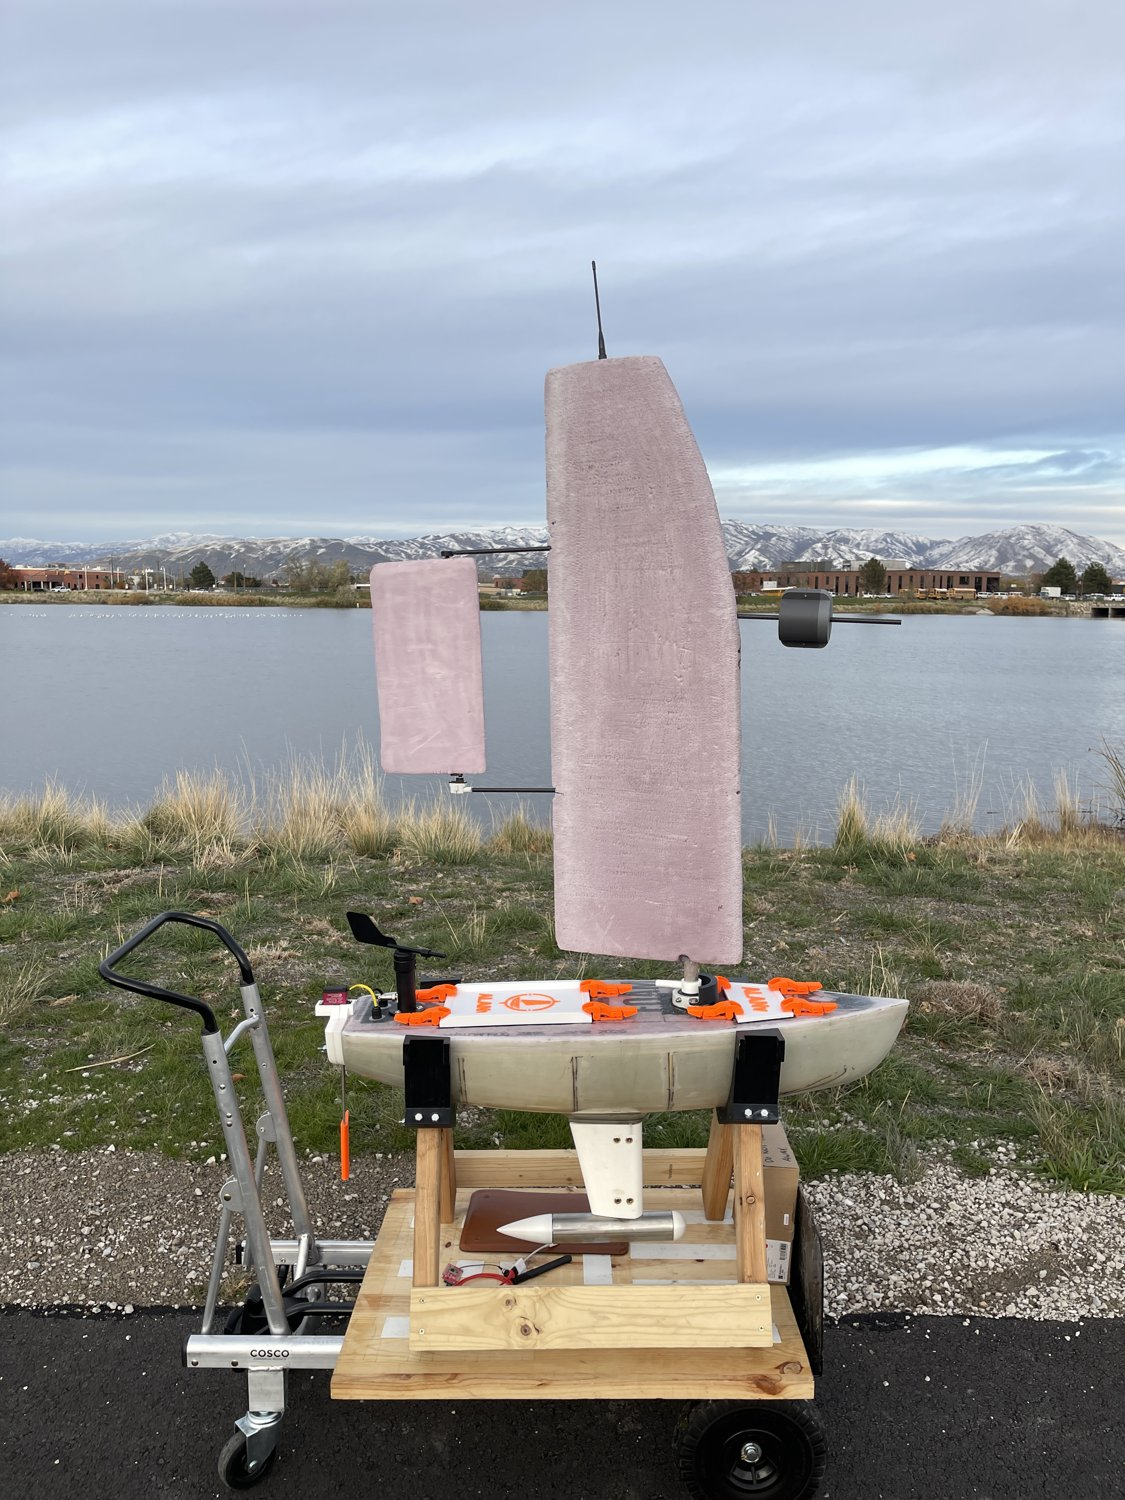
\includegraphics[height=5.6cm]{boat_full}}
\hfil
\subfloat[]{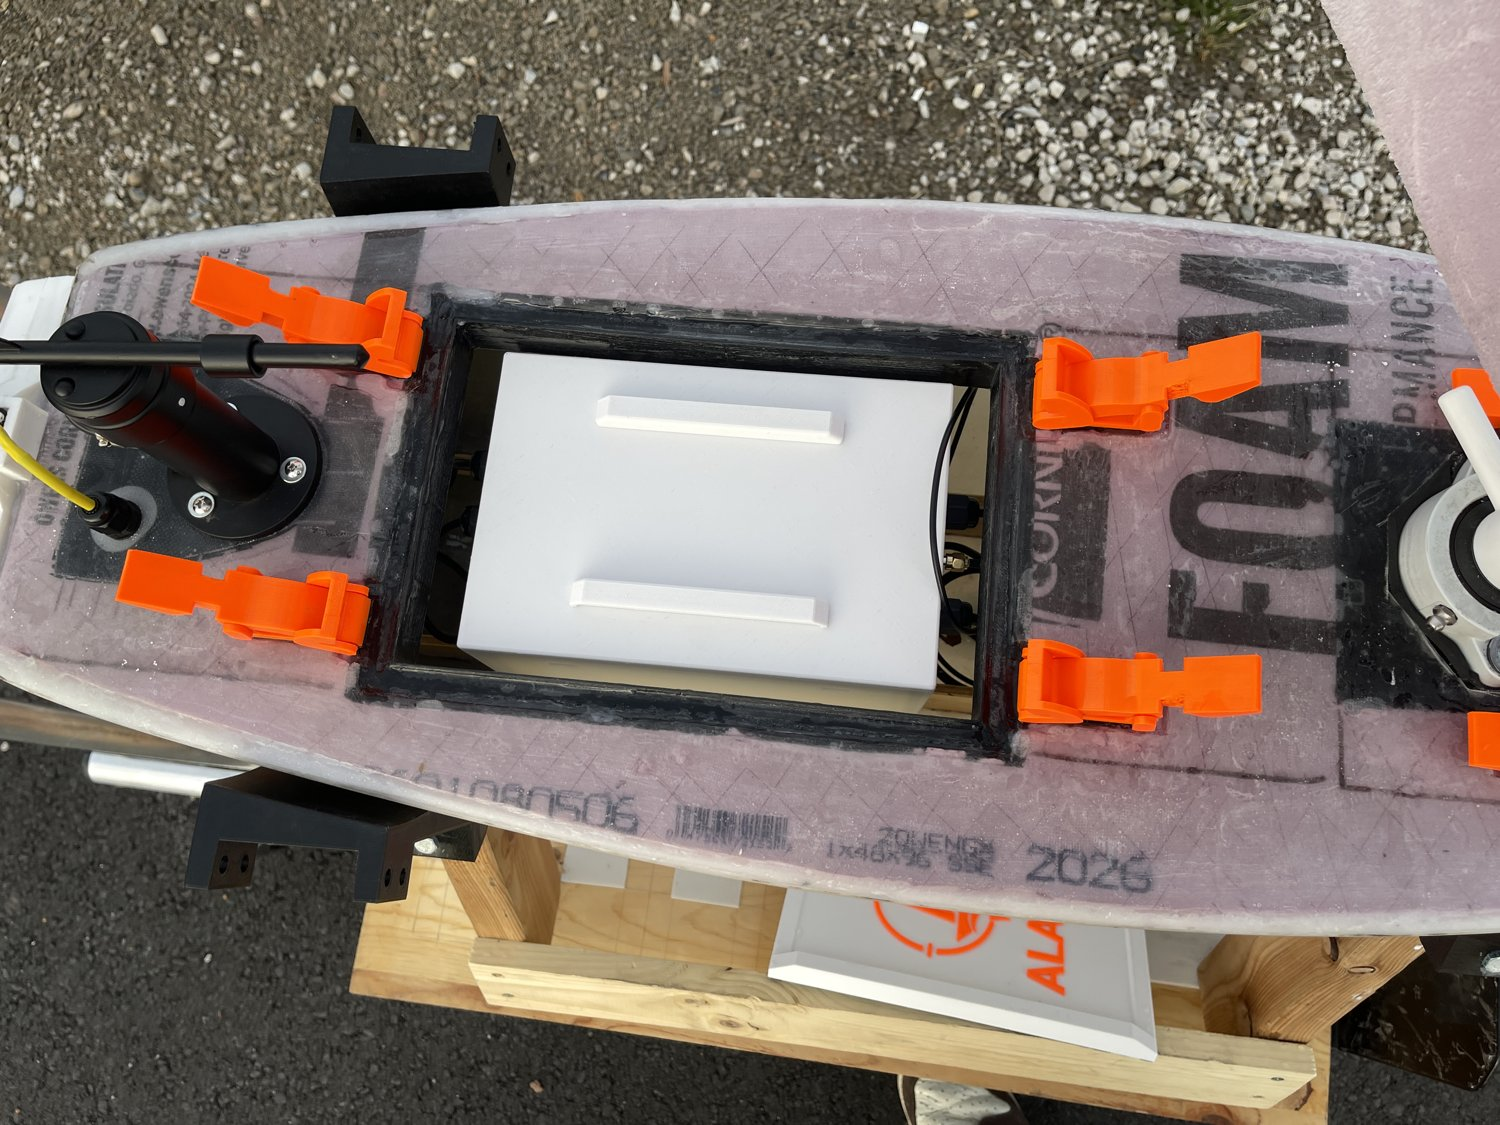
\includegraphics[height=5.6cm]{deck_top}}
\caption{ALAN at the test pond on November 18, 2026. (a) Side view: the
servo-driven tail, the main wing with the LoRa antenna at the masthead, and the
counterweight, with the fin keel and ballast bulb below the hull. (b) Aft deck
from above: the electronics enclosure in its hatch (cover removed), wind vane,
and printed hatch latches.}
\label{fig:boat}
\end{figure*}

\begin{table}[!t]
\caption{Principal Dimensions (from the CAD Model Unless Noted)}
\label{tab:specs}
\centering
\begin{tabular}{@{}lr@{}}
\toprule
Parameter & Value \\
\midrule
Length overall                 & \SI{1.00}{\meter} \\
Beam                           & \SI{0.31}{\meter} \\
Keel depth below hull          & \SI{0.23}{\meter} \\
Mass, ready to sail            & \SI{4.9}{\kilo\gram} (est.) \\
Ballast mass                   & 3.4 {kg} \\
Wing span $\times$ max.\ chord & 1.20 $\times$ \SI{0.35}{\meter} \\
Tail span $\times$ chord       & 0.43 $\times$ \SI{0.22}{\meter} \\
Wing rotation range            & $\pm\SI{90}{\degree}$ \\
Battery                        & \SI{14.8}{\volt} 4S lithium-polymer (LiPo), 1300 mAh \\
\bottomrule
\end{tabular}
\end{table}

\begin{figure*}[!t]
\centering
\begin{tikzpicture}[
  font=\footnotesize,
  blk/.style={draw, rounded corners=2pt, align=center, minimum height=6mm, minimum width=29mm, fill=white},
  core/.style={draw, thick, rounded corners=3pt, align=center, minimum width=48mm, fill=blue!6},
  pwr/.style={draw, rounded corners=2pt, align=center, minimum height=8mm, minimum width=29mm, fill=orange!12},
  data/.style={-{Stealth[length=2mm]}},
  power/.style={-{Stealth[length=2mm]}, orange!80!black, dashed},
  lbl/.style={font=\scriptsize, fill=white, inner sep=1pt}
]
\node[core, minimum height=36mm] (cm7) at (0,0) {\textbf{Cortex-M7} (FreeRTOS)\\[3pt]sensor drivers and orientation fusion\\sail planner (LSP)\\sail and heading PID controllers\\rudder and tail arbiters\\commander (operating modes)\\route manager, telemetry packing};
\node[draw, fill=gray!12, minimum width=48mm, minimum height=7mm, align=center, below=4mm of cm7] (sram) {SRAM4 shared memory: telemetry record, command ring};
\node[core, minimum height=10mm, below=4mm of sram] (cm4) {\textbf{Cortex-M4} (bare metal)\\LoRa driver, \SI{1}{\hertz} telemetry tick};
\begin{scope}[on background layer]
\node[draw, dashed, rounded corners=4pt, inner sep=2.5mm, fit=(cm7)(sram)(cm4),
      label={[font=\scriptsize\itshape, anchor=south]north:STM32H755 on NUCLEO-H755ZI-Q}] (mcu) {};
\end{scope}
\draw[{Stealth[length=2mm]}-{Stealth[length=2mm]}] (cm7) -- (sram);
\draw[{Stealth[length=2mm]}-{Stealth[length=2mm]}] (sram) -- (cm4);
% sensors
\node[blk] (gps)  at (-6.2, 1.40) {GPS receiver};
\node[blk] (imu)  at (-6.2, 0.65) {BNO055 orientation};
\node[blk] (enc)  at (-6.2,-0.10) {AS5600 sail encoder};
\node[blk] (wind) at (-6.2,-0.85) {Wind vane};
\node[blk] (taps) at (-6.2,-1.60) {Battery cell taps};
\draw[data] (gps.east)  -- node[lbl,above]{UART7, NMEA}  (gps.east  -| cm7.west);
\draw[data] (imu.east)  -- node[lbl,above]{I\textsuperscript{2}C2} (imu.east  -| cm7.west);
\draw[data] (enc.east)  -- node[lbl,above]{I\textsuperscript{2}C1} (enc.east  -| cm7.west);
\draw[data] (wind.east) -- node[lbl,above]{UART4, Modbus} (wind.east -| cm7.west);
\draw[data] (taps.east) -- node[lbl,above]{ADC1} (taps.east -| cm7.west);
% actuators
\node[blk] (rud)  at (6.2, 0.9) {Rudder servo};
\node[blk] (tail) at (6.2, 0.0) {Tail servo (in wingsail)};
\draw[data] (rud.west  -| cm7.east) -- node[lbl,above]{TIM1 PWM} (rud.west);
\draw[data] (tail.west -| cm7.east) -- node[lbl,above]{TIM1 PWM} (tail.west);
% radio and ground station
\node[blk] (lora) at (6.2, -3.85) {RFM95W LoRa radio\\915 MHz};
\node[blk, fill=green!8, below=6mm of lora] (gs) {Ground station\\(SAMD21 Pro RF bridge, laptop)};
\draw[{Stealth[length=2mm]}-{Stealth[length=2mm]}] (lora.west -| cm4.east) -- node[lbl,above]{SPI1} (lora.west);
\draw[{Stealth[length=2mm]}-{Stealth[length=2mm]}] (lora) -- node[lbl,right]{RF} (gs);
% power
\node[pwr] (pdb) at (-6.2,-3.0) {Power distribution\\and regulation};
\node[pwr, below=4mm of pdb] (bat) {14.8 V 4S LiPo};
\draw[power] (bat) -- (pdb);
\draw[power] (pdb.east) -- (pdb.east -| mcu.west);
\end{tikzpicture}
\caption{Electrical and software architecture. The CM7 owns all sensing,
control, and actuation; the CM4 owns the radio; the cores communicate only
through shared SRAM4. Solid arrows carry data and dashed arrows carry power.}
\label{fig:block}
\end{figure*}
